\begin{frame}{Simulation Numérique et Maillage : Définition}
  
    \textbf{Simulation Numérique:}
    \begin{itemize}
      \item Technique utilisant des ordinateurs pour reproduire le comportement d'un système via des modèles mathématiques.
      \item Émergence : 1940s (projet Manhattan).
    \end{itemize}
    
    \pause
    \vspace*{.3cm}
    \textbf{Maillage:}
    \begin{itemize}
      \item Division d'un domaine en éléments discrets pour l'analyse numérique.
      \item Émergence : 1950s (Aéronautique, Spatial).
    \end{itemize}
  
\end{frame}

\iffalse
\begin{frame}{Simulation Numérique et Maillage : Exemple}
    \textbf{Propagation d'onde mécanique dans un téléphone}
    %\end{block}
    
    \begin{columns}
        \begin{column}{0.4\textwidth}
            \begin{itemize}
                \item Le maillage facilite la modélisation du stress mécanique.
                \item La qualité du maillage impacte la simulation 
            \end{itemize}
            \begin{center}
                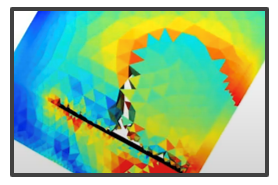
\includegraphics[width=.9\linewidth]{img/new_images/convergence_depend_simu.PNG}
            \end{center}
        \end{column}
        \begin{column}{0.6\textwidth}
            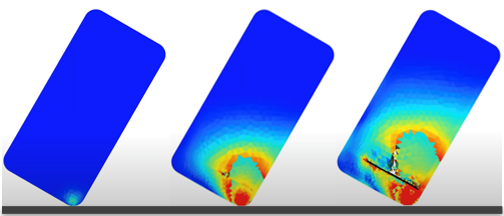
\includegraphics[width=\linewidth]{img/new_images/phone_drop.png}
            \centering
            ANSYS [\cite{kohnke1982ansys}]\\
            %\scriptsize{\url{https://www.youtube.com/watch?v=gVz3eJrMMmM}}
        \end{column}
    \end{columns}
\end{frame}
\fi

\begin{frame}{Pourquoi des maillages quadrilatères / hexaédriques ?}
    \begin{columns}[T] % align columns
        \begin{column}{.4\textwidth}
            \textbf{Pour les simulations de grandes déformations hyper-élastiques :}

            %Pour la mécanique de matériaux hyper-élastiques:
            \begin{itemize}
                \item En 2D, maillage quadrilatère plutôt que triangulaire
                \only<2> {\item En 3D, maillage hexaédrique plutôt que tétraédrique}
            \end{itemize}
        \end{column}%
        
        \begin{column}{.6\textwidth}
            \only<1> {
                \centering \small     
                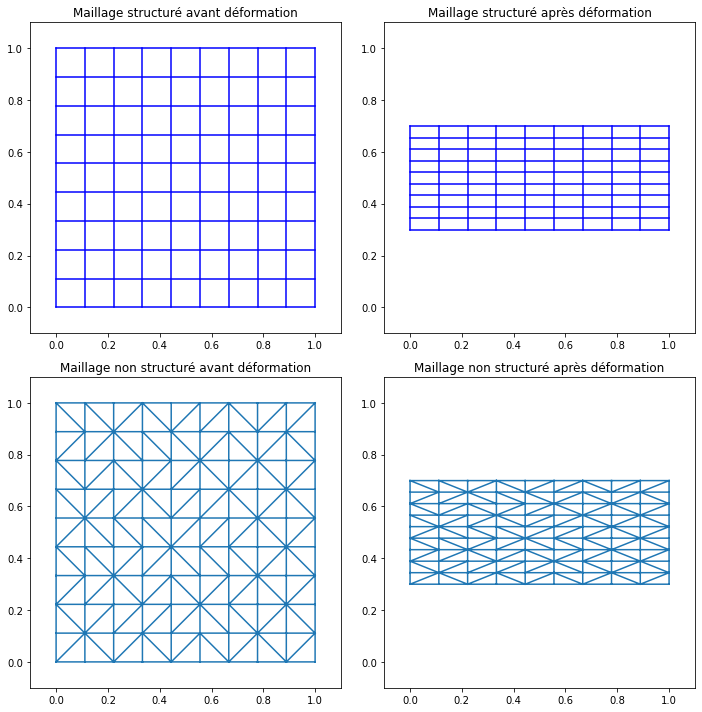
\includegraphics[width=.8\linewidth]{img/choix_maillage/deformation_low_angle.png}\\
                Le maillage quadrilatère préserve des\\ angles de $90^\circ$ malgré la déformation
            }
            \only<2> {
                \centering \small     
                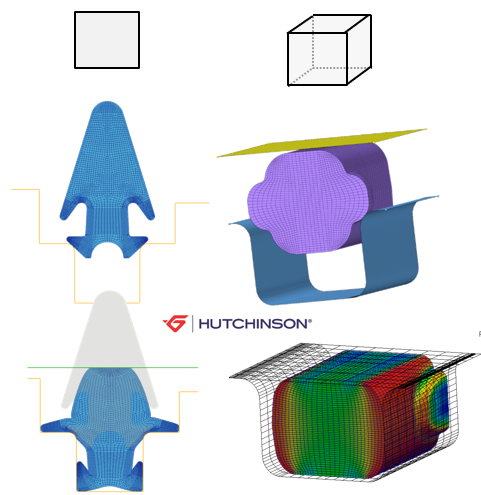
\includegraphics[width=.8\linewidth]{img/new_images/simu_hutchinson_2d3d.png}\\
                Simulation de déformation de joints\\ en caoutchouc par Hutchinson
            }
        \end{column}
    \end{columns}
\end{frame}




